\documentclass[11pt]{article}
\usepackage{amsmath, amssymb}
\usepackage[margin=1in]{geometry}
\usepackage{enumitem}
\usepackage{graphicx}
\setlength{\parindent}{0pt}
\setlength{\parskip}{6pt}

\title{Insights from \texttt{Detect\_Motion\_Starter}\\[2pt]
\large the existing Activity-State baseline (Synheart Kinematics)}
\date{}

\begin{document}
\maketitle

Short notes on the starter notebook --- what it does, what it gets right, and
what it misses. It trains six sklearn models on the $561$ precomputed UCI-HAR
features; the RBF SVM is its best, reported at $97.93\%$.

\section{The headline accuracy is on an easier 4-class problem}
In the cleaning step the three walking types (\textsc{walking},
\textsc{upstairs}, \textsc{downstairs}) are merged into a single \textsc{moving}
class, and the models are trained on that label. So the reported number is
\textbf{4-class} (\textsc{moving}/\textsc{sitting}/\textsc{standing}/\textsc{laying}),
not the standard 6-class UCI-HAR benchmark people quote.

Same model (RBF SVM), measured here:
\begin{itemize}[noitemsep]
  \item 6-class (standard): $95.05\%$
  \item 4-class (his merge): $97.22\%$
\end{itemize}
The merge \emph{removes} the hardest part --- telling the walking types apart ---
instead of solving it. In the 6-class case the errors sit almost entirely in
downstairs/upstairs and sitting/standing; laying has $0$ errors.

\section{No orientation or placement test}
The notebook assumes the phone stays on the waist in one orientation, which is how
UCI-HAR was recorded. There is no rotation or placement check. For a wearable worn
at any angle this is the main gap: rebuilding the same model family on per-axis
features and applying a random phone rotation (Fig.~\ref{fig:henok}, right) drops
it from $92.2\%$ to $26.6\%$ --- a 66-point collapse.

\section{The notebook already holds both the robust and the fragile feature}
Its own EDA shows the acceleration \emph{magnitude} \texttt{tBodyAccMagmean}
(orientation-proof) cleanly splits moving vs stationary, while at the same time it
uses the gravity-\emph{angle} \texttt{angleXgravityMean} (orientation-dependent) to
pick out laying. The two are never distinguished --- but one survives a rotation and
the other does not. That distinction is the whole point of the task.

\section{Small bugs}
\begin{itemize}[noitemsep]
  \item t-SNE marker list has $6$ markers for the $4$-class data (errors out).
  \item Confusion-matrix labels are hardcoded to $6$ names for a $4$-class model.
  \item The Gradient-Boosting grid includes invalid $0$ values and is $\sim 700$ fits.
\end{itemize}

\section{Fit to the assignment}
$561$ features is not lightweight or on-device-friendly, and many are
orientation-coupled ($303$ per-axis $+\,7$ gravity-angle). The brief asks for the
opposite: few features, lightweight, orientation-proof.

\emph{Fair credit:} the official train/test split he uses \emph{is}
subject-independent (different volunteers in the test set), so his score does
generalize across people. The weakness is orientation and the 4-class shortcut,
not person-leakage.

\begin{figure}[h]
\centering
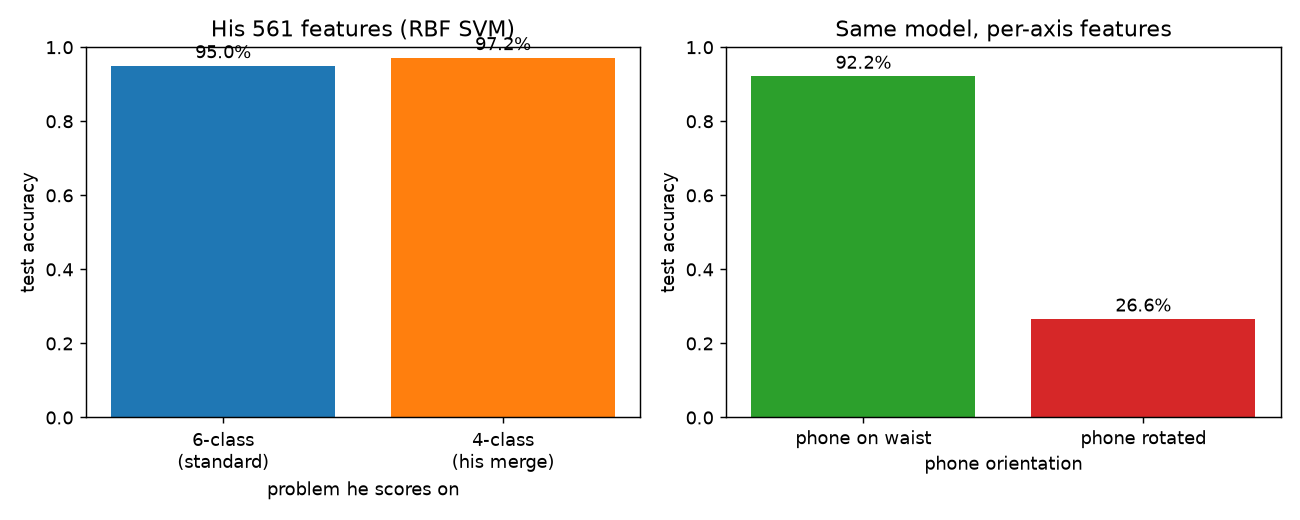
\includegraphics[width=\textwidth]{figs/fig_henok.png}
\caption{Left: his RBF SVM on the $561$ features --- the 4-class merge he trains on
scores higher than the standard 6-class. Right: the same model family on per-axis
features, scored on the waist data vs after a random phone rotation.}
\label{fig:henok}
\end{figure}

\end{document}
